\section{Sacred Science 106: Origin of Mind}

Being is One, yet it contains within itself multiplicity, since it produces it by the deployment of its possibilities alone. Purusha (Essence) and Prakriti (Substance) are the two poles that bring these possibilities into manifestation.

Prakriti contains all possibilities of manifestation as known by Purusha, so it is the first principle of manifestation. Prakriti is passive and purely potential so that it cannot be a cause in itself. That means that intelligence comes prior to any sort of manifestation.

\begin{figure}[t]
\centering
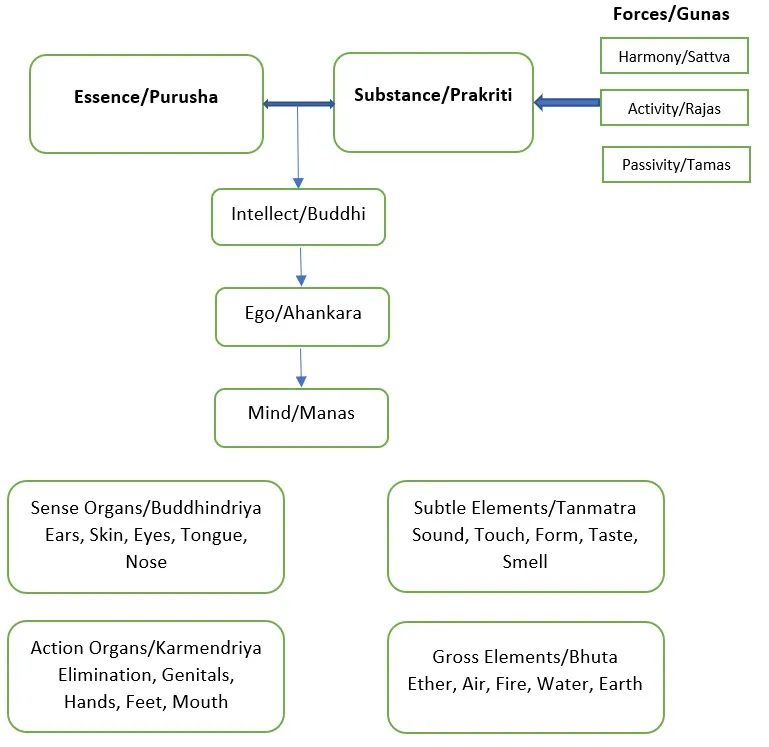
\includegraphics[scale=.35]{SamkhyaChart.png}
\caption{Samkhya Chart}
\end{figure} 

In Western terms, Purusha is Essence and Prakriti is Substance. The union of Essence and Substance is called hylomorphism. This is not dualistic in the Cartesian sense. Rather it recognizes that there is both an inside and an outside to the world, the former as the subtle state and the latter as the gross state. The understanding of the multiple states of the being avoids philosophical conundrums like explaining the relationship between consciousness and matter, or how they interact.

\paragraph{Intellect}
The first production of Purusha and second principal is the Intellect (Buddhi). Although manifested, it is formless.

Thus, there cannot be any direct experience of it. The Intellect is of a transcendent order and has the knowledge of universal principles as its proper object. This knowledge, which is not discursive, is obtained directly and immediately by intellectual intuition.

There are stories about direct intuition of the Intellect. For example, mystics, composers, poets, philosophers, visionaries, etc., have often reported that their greatest works just “came to them”, as if from the outside. The mathematician, Ramanujan, claimed that a goddess revealed all his mathematical discoveries to him. Their task, then, was just to write down their inspirations.

Perhaps, you’ve had a similar experience on a smaller scale. Often that is called the “aha experience”. Suppose you have been working on a mathematical problem without understanding, but then suddenly you just “get it”.

\paragraph{Ego}
The Intellect is the intermediary between personality and individuality. The formless Intellect produces the individual consciousness, or the Ego. As the essences in the Intellect give rise to thought, evoking the notion of the Ego or “I am”.

The Ego becomes concerned with external and internal objects, which are respectively the objects of perception and of contemplation, or in other words, the subtle states and the gross state.

\paragraph{Mind}
Mind, or Manas, is related to individual thought, including reason as well as memory and imagination. In the West, this includes the Five Wits: memory, estimation, fantasy, imagination, and common sense.

The Mind is part of the subtle realm, yet it is the intermediary between the organs of sensation and action. The lowest part of the mind is involved with the senses and the organs of action.

\paragraph{Organs}
These organs allow the human being to both sense and act upon the world.

The Sense Organs or Buddhindriyas are produced in order to experience the subtle states. For the human being, these are the Ears, Skin, Eyes, Tongue, and Nose. They correspond to the senses.

The organs of action are the Karmendriyas. These are the faculties of action such as execratory organs, reproduction, manipulation, locomotion, and speech or ingestion. These are general conditions of life and are found in almost all forms of animal life. For the human being, they are the anus, the genitals, arms, legs, and mouth.

\paragraph{Subtle Elements}
The subtle elements, or Tanmatras, are Sound, Touch, Form, Taste, and Smell. Together they form the inner experience of the world.

Although these are not experienced outwardly, that does not indicate that they are merely subjective experiences. They are as much a part of the world as are the gross elements.

\paragraph{Gross Elements}
The gross elements, or bhutas, are ether, air, fire, water, and earth which correspond to the subtle experiences: auditory, tangible, visible, sapid, and olfactory.

Note that the gross elements are the very last productions of prakriti. Together, they form what is called “matter” by science and in common usage. The material world, in itself, does not have any sensible qualities. Galileo made it explicit: secondary qualities (such as sense experience) are not part of science. For example, all the theories and equations of science do not require the notion of color, nor any other subtle element.

For science, matter is characterized by number, extension, solidity or mass, and motion. The subtle elements are the principle of the gross elements, but matter is the principle of multiplicity. In matter, there can be multiple instances of the same essence.

Ether can also be understood as space, so matter has extension in space as well as shape.

Earth represents mass and fire the energy associated with motion. Air and water round out the other states of experienceable matter.

Since matter is closest to Prakriti, it takes on some of its characteristics. For example, matter includes three forces, usually expressed by the terms positive, negative, and neutral.

Prime matter, similar to Prakriti, is passive and malleable. Quantum indeterminacy is analogous to the receptivity of Prakriti. Vertical causation, i.e., the influence of Purusha on Prakriti ends indeterminacy so that individual things are formed.

Profane science believes that the matter of the gross state is fundamental and so that all the productions are caused by matter. This includes the senses, the mind, thoughts, the Ego, and Intelligence. Random evolution brings the organs of sense and activity into existence. But if matter has no secondary qualities, what is the purpose of the evolution of the eye to “see” something that simply isn’t there?

The scientific view implies that all the possibilities of manifestation are hidden in matter somewhere. There is certainly no compelling reason to believe that and no physical theory can explain it.

Some claim that “emergent evolution” offers an explanation, but that just means that there must be something higher than matter, in order for new qualities to arise.

\flrightit{Posted on 2022-10-27 by Cologero}

\begin{center}* * *\end{center}

\begin{footnotesize}\begin{sffamily}

\texttt{Rui Artur on 2022-10-28 at 10:03 said: }

It might be useful to note in the text – for those who wish to go forth and link this to the Western Tradition – that in texts from the Latin part of the world one will encounter the idea of Purusha coming from the Greek ousia but translated as ‘substance’ (rather than ‘essence’). This can cause some confusion if one is not reading carefully or just beginning his study, even though ‘essence’ is etymologically correct and substance is not (which is why I think Guenon used it).

\hfill

\texttt{Balder on 2022-10-30 at 09:57 said: }

I have related the Nordic conception of Ginnun-Ga-Gap as the Absolute (greek Khaos) and Fire representing Essence/Purusha and Ice Substance/Prakriti. There is a fine thread uniting Hindu metaphysics, indo-European Cultural connexion and Norse / Finno-Ugric / European Pagan metaphysics.

\hfill

\texttt{Balder on 2022-10-30 at 10:03 said: }

In the Finno-Ugric tradition the same concepts are Lintukoto (The Birdlands) and Pohjola (The Northlands).

In the Norse tradition the trinity Odin-Vili-Ve represent the threefold structure of buddhi-ahamkara-manas.They are the “first creator Gods” to emerge from the primordial chaos and they slay Ymir, who is here Purusha personified. Essence is “slayed” or crucified into the Cross of matter.

\hfill

\texttt{Cologero on 2022-10-31 at 17:14 said: }

This is a work in progress, and some things, particularly terminology, will have to be reviewed.

\hfill

\end{sffamily}\end{footnotesize}